\documentclass{beamer}

\usepackage{amssymb,amsmath}
\usepackage{graphicx}
\usepackage{url}
\usepackage{color}
\usepackage{relsize}		% For \smaller
\usepackage{url}			% For \url
\usepackage{epstopdf}	% Included EPS files automatically converted to PDF to include with pdflatex

%For MindMaps
% \usepackage{tikz}%
% \usetikzlibrary{mindmap,trees,arrows}%

%%% Color Definitions %%%%%%%%%%%%%%%%%%%%%%%%%%%%%%%%%%%%%%%%%%%%%%%%%%%%%%%%%
%\definecolor{bordercol}{RGB}{40,40,40}
%\definecolor{headercol1}{RGB}{186,215,230}
%\definecolor{headercol2}{RGB}{80,80,80}
%\definecolor{headerfontcol}{RGB}{0,0,0}
%\definecolor{boxcolor}{RGB}{186,215,230}

%%% Save space in lists. Use this after the opening of the list %%%%%%%%%%%%%%%%
%\newcommand{\compresslist}{
%	\setlength{\itemsep}{1pt}
%	\setlength{\parskip}{0pt}
%	\setlength{\parsep}{0pt}
%}

%\setbeameroption{show notes on top}

% You should run 'pdflatex' TWICE, because of TOC issues.

% Rename this file.  A common temptation for first-time slide makers
% is to name it something like ``my_talk.tex'' or
% ``john_doe_talk.tex'' or even ``discrete_math_seminar_talk.tex''.
% You really won't like any of these titles the second time you give a
% talk.  Try naming your tex file something more descriptive, like
% ``riemann_hypothesis_short_proof_talk.tex''.  Even better (in case
% you recycle 99% of a talk, but still want to change a little, and
% retain copies of each), how about
% ``riemann_hypothesis_short_proof_MIT-Colloquium.2000-01-01.tex''?

\mode<presentation>
{
  % A tip: pick a theme you like first, and THEN modify the color theme, and then add math content.
  % Warsaw is the theme selected by default in Beamer's installation sample files.

  %%%%%%%%%%%%%%%%%%%%%%%%%%%% THEME
  %\usetheme{AnnArbor}
  %\usetheme{Antibes}
  %\usetheme{Bergen}
  %\usetheme{Berkeley}		% bem bacana - menu esquerdo
  %\usetheme{Berlin}
  %\usetheme{Boadilla}
  %\usetheme{boxes}
  %\usetheme{CambridgeUS}		% bem bacana - menu superior
  %\usetheme{Copenhagen}
  %\usetheme{Darmstadt}
  %\usetheme{default}
  %\usetheme{Dresden}
  \usetheme{Frankfurt}
  %\usetheme{Goettingen}
  %\usetheme{Hannover}		% bem bacana - menu esquerdo
  %\usetheme{Ilmenau}
  %\usetheme{JuanLesPins}
  %\usetheme{Luebeck}
  %\usetheme{Madrid}		%bacana
  %\usetheme{Malmoe}
  %\usetheme{Marburg}		% bem bacana - menu direito
  %\usetheme{Montpellier}
  %\usetheme{PaloAlto}		% bem bacana - menu esquerdo
  %\usetheme{Pittsburgh}
  %\usetheme{Rochester}		%bacana
  %\usetheme{Singapore}
  %\usetheme{Szeged}
  %\usetheme{Warsaw}

  %%%%%%%%%%%%%%%%%%%%%%%%%%%% COLOR THEME
  %\usecolortheme{albatross}		% azul escuro, massa
  %\usecolortheme{beetle}		% cinza, menu azul
  %\usecolortheme{crane}		% branco e amarelo, massa
  \usecolortheme{default}		% branco, azul clarinho
  %\usecolortheme{dolphin}		% azul e branco, legal
  %\usecolortheme{dove}			% cinza e branco, feio
  %\usecolortheme{fly}			% todo cinza, horrível
  %\usecolortheme{lily}			% parece o default
  %\usecolortheme{orchid}		% azul e branco, ok
  %\usecolortheme{rose}			% branco e violeta-claro, bonito
  %\usecolortheme{seagull}		% cinza, feio
  %\usecolortheme{seahorse}		% nhé, meio feio
  %\usecolortheme{sidebartab}		% Azul, branco, destaque na tab, interessante
  %\usecolortheme{structure}		% bichado
  %\usecolortheme{whale}		% Azul e branco, bem bonito

  %%%%%%%%%%%%%%%%%%%%%%%%%%%% OUTER THEME
  \useoutertheme{default}
  %\useoutertheme{infolines}
  %\useoutertheme{miniframes}
  %\useoutertheme{shadow}
  %\useoutertheme{sidebar}
  %\useoutertheme{smoothbars}
  %\useoutertheme{smoothtree}
  %\useoutertheme{split}
  %\useoutertheme{tree}

  %%%%%%%%%%%%%%%%%%%%%%%%%%%% INNER THEME
  \useinnertheme{circles}
  %\useinnertheme{default}
  %\useinnertheme{inmargin}
  %\useinnertheme{rectangles}
  %\useinnertheme{rounded}

  %%%%%%%%%%%%%%%%%%%%%%%%%%%%%%%%%%%

  \setbeamercovered{invisible} % or whatever (possibly just delete it)
  % To change behavior of \uncover from graying out to totally
  % invisible, can change \setbeamercovered to invisible instead of
  % transparent. apparently there are also 'dynamic' modes that make
  % the amount of graying depend on how long it'll take until the
  % thing is uncovered.

}


% Get rid of nav bar
\beamertemplatenavigationsymbolsempty

% Use short top
%\usepackage[headheight=12pt,footheight=12pt]{beamerthemeboxes}
%\addheadboxtemplate{\color{black}}{
%\hskip0.5cm
%\color{white}
%\insertshortauthor \ \ \ \ 
%\insertframenumber \ \ \ \ \ \ \ 
%\insertsection \ \ \ \ \ \ \ \ \ \ \ \ \ \ \ \ \  \insertsubsection
%\hskip0.5cm}
%\addheadboxtemplate{\color{black}}{
%\color{white}
%\ \ \ \ 
%\insertsection
%}
%\addheadboxtemplate{\color{black}}{
%\color{white}
%\ \ \ \ 
%\insertsubsection
%}

% Insert frame number at bottom of the page.
% \usefoottemplate{\hfil\tiny{\color{black!90}\insertframenumber}} 

\usepackage[english]{babel}
\usepackage[latin1]{inputenc}
\usepackage{subfigure}

\usepackage{times}
\usepackage[T1]{fontenc}

\usepackage{tikz}
\usetikzlibrary{arrows,shapes}
% Latex Graph Example:
% https://www.overleaf.com/5297501zrjzfm#/16716638/

% TODO: Silly Makefile

\tikzstyle{vertex}=[circle,fill=black!25,minimum size=10pt,inner sep=0pt]
\tikzstyle{blue vertex}=[circle,fill=blue!100,minimum size=10pt,inner sep=0pt]
\tikzstyle{red vertex}=[circle,fill=red!100,minimum size=10pt,inner sep=0pt]
\tikzstyle{edge} = [draw,thick,-]
\tikzstyle{red edge} = [draw, line width=5pt,-,red!50]
\tikzstyle{black edge} = [draw, line width=5pt,-,black!20]
\tikzstyle{weight} = [font=\smaller]

\title[GB21802]{GB21802 - Programming Challenges}
\subtitle[]{Week 6 - Graph Problems (Part II)}
\author[Claus Aranha]{Claus Aranha\\{\footnotesize caranha@cs.tsukuba.ac.jp}}
\institute{College of Information Science}
\date{2015-06-03,6\\{\tiny Last updated \today}}

\begin{document}

\section{Introduction}
\subsection{Title}
\begin{frame}
\maketitle
\end{frame}

\subsection{Notes and Warnings}

\begin{frame}
  \frametitle{Last Week Results}
  \begin{block}{Week 5 - Graph I}
  \begin{columns}[T]
    \column{0.5\textwidth}
    \begin{itemize}
    \item Denominator -- 17/31
    \item Knight War Grid -- 10/31
    \item Wetlands of Florida -- 8/31
    \item Battleships -- 3/31
    \item Pick up Sticks -- 1/31
    \end{itemize}
    \column{0.5\textwidth}
    \begin{itemize}
    \item Place the Guards -- 1/31
    \item Street Dominos -- 0/31
    \item Dominos -- 0/31
    \item Freckles -- 5/31
    \item Artic Network -- 0/31
    \end{itemize}
  \end{columns}

  \medskip
  {\smaller
    \begin{itemize}
      \item 10 people solved: 0 problems;
      \item 7 people solved: 1 problem;
      \item 3 people solved: 2 problems;
      \item 10 people solved: 3-4 problems;
      \item 1 person solved: 7 problems!
    \end{itemize}
  }
  \end{block}
\end{frame}

\begin{frame}
  \frametitle{Special Notes}
  
\end{frame}

\begin{frame}
  \frametitle{Week 5 and 6 -- Outline}
  {\smaller
  \begin{block}{Last Week - Graph I}
    \begin{itemize}
    \item Graph Basics review: Concepts and Data Structure;
    \item Depth First Search and Breadth First Search;
    \item Problems you solve with DFS and BFS;
    \item Minimum Spanning Tree: Kruskal and Prim Algorithms;
     \end{itemize}
  \end{block}
  \begin{block}{Next Week - Graph II}
    \begin{itemize}
    \item Single Sourse Shortest Path; (Friday)
    \item All Pairs Shortest Path; (Friday)
    \item Network Flow; (Monday)
    \item Special Graphs and Related Problems; (Monday)
    \end{itemize}
  \end{block}}
  Many variations in graph problems!
\end{frame}

\section{SSSP}
\subsection{Single Source Shortest Path}
\begin{frame}
  \frametitle{SSSP: Single Source Shortest Path}
  {\smaller
    \begin{block}{Problem Definition}
      Given a graph $G$ and a source $s$, what
      are the shortest paths from $s$ to a target node $t$?
    \end{block}

    \bigskip

    Common solutions:

    \begin{itemize}
    \item On \alert{unweighted} graphs, BFS is good enough, but it
      won't work correctly in weighted graphs;
    \item Djikstra Algorithm (usually $O((V+E)\text{log}V)$)
    \item Bellman Ford's Algorithm $O(VE)$
    \end{itemize}
  }
\end{frame}

\begin{frame}[fragile,singleslide]
  \frametitle{Reminder: SSSP on unweighted graph (BFS)}

{\smaller
    \begin{itemize}
    \item Visit nodes from $s$ to $t$;
    \item Calculate minimal cost from $s$ to $t$;
    \item (optional) Print the path from $s$ to $t$;
    \end{itemize}

\begin{exampleblock}{}
\begin{verbatim}
vector <int> p; // list of parents
void printPath(u) { // recursive print path s to u
   if (u == s) { cout << s; return; } // base case
   printPath(p[u]); cout << " " << u; }

vector <int> dist(V,INF); dist[s] = 0;
queue <int> q; q.push(s);
while (!q.empty()) {
   int u = q.front(); q.pop();
   for (int j = 0; j < (int)AdjList[u].size(); j++) {
      pair <int,int> v = AdjList[u][j];
      if (dist[v.first] == INF) { 
         dist[v.first] = dist[u] + 1;
         p[v.first] = u; q.push(v.first); }}}
\end{verbatim}
\end{exampleblock}
}
\end{frame}

\begin{frame}
  \frametitle{BFS: Problem with weighted graphs}

  \begin{block}{}
    Simple BFS will give a wrong answer when there is a longer path
    which is cheaper than a shorter one.
  \end{block}
  
  \medskip

  \begin{center}
    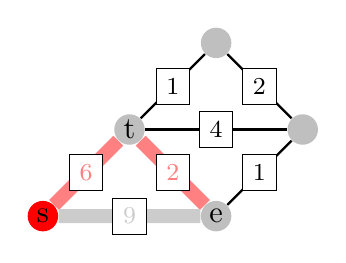
\begin{tikzpicture}[transform shape,label/.style={thin, draw=black, align=center,fill=white,font=\smaller},scale=1.1]
      \node[vertex] (a) at (0,0) {t};
      \node[vertex] (b) at (1,1) {};
      \node[vertex] (c) at (2,0) {};
      \node[vertex] (d) at (1,-1) {e};
      \node[red vertex] (e) at (-1,-1) {s};
      \draw[edge] (a) -- node[label] {$1$} (b);
      \draw[edge] (b) -- node[label] {$2$} (c);
      \draw[edge] (a) -- node[label] {$4$} (c);
      \draw[red edge] (a) -- node[label] {$2$} (d);
      \draw[edge] (c) -- node[label] {$1$} (d);
      \draw[red edge] (a) -- node[label] {$6$} (e);
      \draw[black edge] (d) -- node[label] {$9$} (e);
    \end{tikzpicture}
  \end{center}

  \bigskip

  In this graph, BFS would find $s \rightarrow e$ (cost 9) as the
  shortest path from $s$ to $e$, instead of $s \rightarrow t
  \rightarrow e$ (cost 8).
\end{frame}

\subsection{SSSP with Weighted Graph}
\begin{frame}
  \frametitle{Djikstra's Algorithm for weighted SSSP}
  \begin{block}{Basic Idea}
    Greedly selects the next edge that minimizes the total weight of the visited graph.
  \end{block}

  {\small
  \begin{itemize}
  \item Many different implementations (original paper has no implementation);
  \item A simple way is to use C++ stl's \emph{Priority Queue};
  \item When visiting a node, store new edges in the priority queue;
    {\smaller (priority queue sort edges as they are inserted)}
  \item For every new edge visited, check if new path on target node
    is cheaper than old one (if it is cheaper, visit the node again);
  \end{itemize}}
\end{frame}

\begin{frame}[fragile,singleslide]
  \frametitle{Djikstra's Algorithm: \_A\_ Implementation}
  {\smaller
    \begin{exampleblock}{}
\begin{verbatim}
Vector<int> dist(V,INF); dist[s] = 0;
priority_queue<ii, vector<ii>, greater<ii>> pq; 
pq.push(ii,(0,s));
while (!pq.empty()) {
   ii front = pq.top(); pq.pop(); 
   // shortest unvisited vertex
   int d = front.first; u = front.second;
   if (d > dist[u]) continue; // *lazy deletion*
   for (int j = 0; j < (int)AdjList[u].size(); j++) { 
      ii v = AdjList[u][j];
      if (dist[u] + v.second < dist[v.first]) { 
         dist[v.first] = dist[u] + v.second // relax
         pq.push(ii(dist[v.first],v.first));}}} 
         // new node to queue
\end{verbatim}
    \end{exampleblock}

    This implementation uses \emph{lazy deletion} to avoid deleting
    nodes from the queue unless absolutely necessary;}
\end{frame}

\begin{frame}
  \frametitle{Djikstra's implementation trick: Lazy deletion}
  {\smaller
    \begin{itemize}
    \item Djikstra Requires us to store the edge to vertex $v$ with
      cheapest weight in the queue;
    \item Removing an edge from the queue is expensive;
    \item Instead, we keep all edges, and test each visited edge;
    \end{itemize}
  

  % TODO: Redraw Djikstra graph by hand
  \begin{center}
    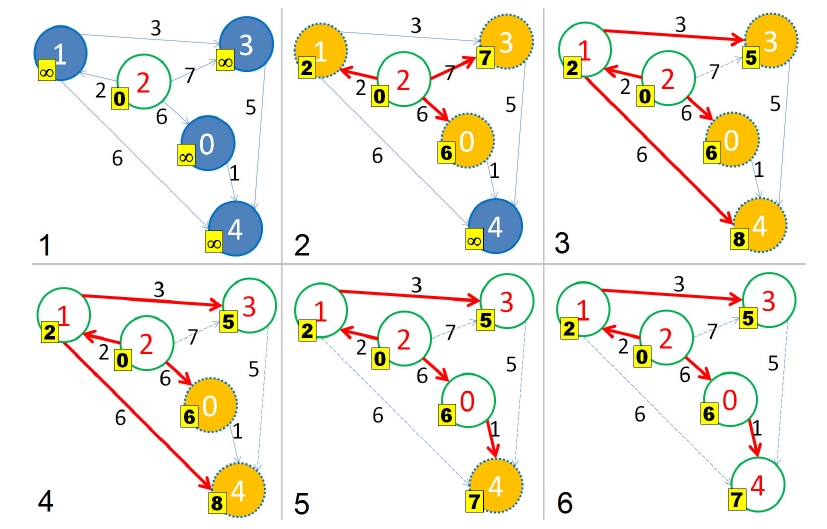
\includegraphics[width=0.6\textwidth]{../img/djikstra_halim}
  \end{center}

  Vertex queue: [\only<1>{(2,1),}\only<2>{(5,3),}
    \only<1-3>{(6,0),}\only<1-4>{(7,3),}
    \only<4->{(7,4),}\only<2->{(8,4),} \only<3->{(10,4)}];}

  \vfill 

  \hfill {\tiny Images from \emph{Competitive Programming}, Steven Halim}
\end{frame}

\subsection{Example: Full Tank?}
\begin{frame}
  \frametitle{Problem Example: UVA 11367 -- Full Tank} 
  {\smaller 
    A big part of Graph problems is figuring out the correct graph
    representation.

  \begin{block}{Problem Summary}
    In a graph $G$ of roads ($1 \leq V \leq 1000, 0 \leq E \leq
    10000$) with the following information:
    \begin{itemize}
    \item cost $l_{ij}$ in units of fuel between cities $i$ and $j$;
    \item price $p_{i}$ of buying fuel at city $i$;
    \item tank capacity $c$ of a car;
    \end{itemize}
    What is the least \structure{fuel price} from node $s$ to $e$; 
  \end{block}
  
   \begin{center}
    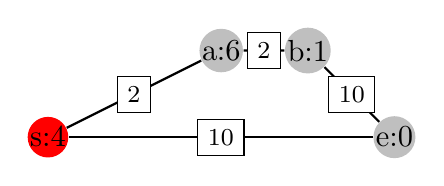
\begin{tikzpicture}[transform shape,label/.style={thin, draw=black, align=center,fill=white,font=\smaller},scale=1.1]
      \node[red vertex] (s) at (0,0) {s:4};
      \node[vertex] (0) at (2,1) {a:6};
      \node[vertex] (1) at (3,1) {b:1};
      \node[vertex] (e) at (4,0) {e:0};
      \draw[edge] (s) -- node[label] {$10$} (e);
      \draw[edge] (s) -- node[label] {$2$} (0);
      \draw[edge] (0) -- node[label] {$2$} (1);
      \draw[edge] (1) -- node[label] {$10$} (e);
    \end{tikzpicture}
  \end{center}
  
   The regular shortest path is $s$ to $e$, but the smallest fuel
   price is buying fuel at $s$ (cost 4) and at $a$ (cost 1), for a total cost 26}
\end{frame}

\begin{frame}
  \frametitle{UVA 11367 -- Full Tank -- Problem modeling}
  {\smaller
    \begin{center}
      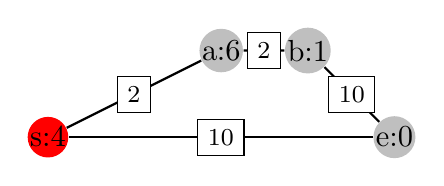
\begin{tikzpicture}[transform shape,label/.style={thin, draw=black, align=center,fill=white,font=\smaller},scale=1.1]
        \node[red vertex] (s) at (0,0) {s:4};
        \node[vertex] (0) at (2,1) {a:6};
        \node[vertex] (1) at (3,1) {b:1};
        \node[vertex] (e) at (4,0) {e:0};
        \draw[edge] (s) -- node[label] {$10$} (e);
        \draw[edge] (s) -- node[label] {$2$} (0);
        \draw[edge] (0) -- node[label] {$2$} (1);
      \draw[edge] (1) -- node[label] {$10$} (e);
      \end{tikzpicture}
    \end{center}
    
    \begin{block}{}
    Simple Djikstra on the $l_{ij}$ graph will not solve this problem,
    because we have to take into account the cost of buying fuel at
    different nodes.
    \end{block}
    
    \bigskip
    
    To model this problem, we modify the graph:
    \begin{itemize}
    \item Transform nodes $(i)$ into nodes $(i,f)$ (how much fuel left
      we have at $i$);
    \item An edge $(i,f)\rightarrow(j,f-l_{ij})$ exists if $f-l_{ij}
      \geq 0$ and has cost 0 (spend existing fuel);
    \item An edge $(i,f)\rightarrow(i,f+1)$ has cost $p_i$ (buy fuel at the city)
    \item Use regular djikstra on the new graph;
    \end{itemize}

  }
\end{frame}

\subsection{SSSP with Negative Cycle}
\begin{frame}
  \frametitle{Djikstra Problem with negative cycles}

  {\smaller
    \begin{block}{}
      The djikstra implementation suggested earlier \structure{can deal}
      with negative weights, but will enter an infinite loop if the graph
      has a \alert{negative loop}.
    \end{block}

    \begin{center}
      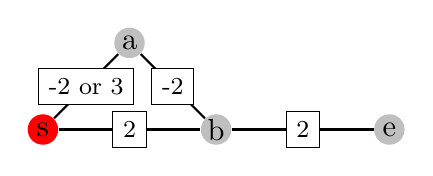
\begin{tikzpicture}[transform shape,label/.style={thin, draw=black, align=center,fill=white,font=\smaller},scale=1.1]
        \node[red vertex] (s) at (0,0) {s};
        \node[vertex] (0) at (1,1) {a};
        \node[vertex] (1) at (2,0) {b};
        \node[vertex] (e) at (4,0) {e};
        \draw[edge] (s) -- node[label] {-2 or 3} (0);
        \draw[edge] (s) -- node[label] {2} (1);
        \draw[edge] (1) -- node[label] {-2} (0);
      \draw[edge] (1) -- node[label] {2} (e);
      \end{tikzpicture}
    \end{center}
    
    \begin{itemize}
    \item The Djikstra implementation above will keep adding negative
      nodes as smaller totals are generated: -2, -4, -6, -8...
    \item The Problem is that it does not include an explicit check
      for \emph{non-simple} paths;
    \item To deal with negative loops, one alternative is the
      \structure{Bellman Ford's algorithm}
    \end{itemize}
  }
\end{frame}

\begin{frame}[fragile,singleslide]
  \frametitle{Bellman Ford's Algorithm $O(VE)$}

  {\smaller
  \structure{Main Idea}: Relax all $E$ edges in the graph $V-1$ times;

  \begin{exampleblock}{}
\begin{verbatim}
vector<int> dist(V, INF); dist[s] = 0;
for (int i = 0; i < V - 1; i++) // repeat V-1 times
 for (int u = 0; u < V; u++) // for all vertices
  for (int j = 0; j < (int)AdjList[u].size(); j++) {
    ii v = AdjList[u][j]; // record path here if needed;
    dist[v.first] = min(dist[v.first], dist[u]+v.second);
    } //relax edge
\end{verbatim}
  \end{exampleblock}
  
  \medskip

  \structure{How does it work?}:
  \begin{itemize}
  \item At the start, \emph{dist[s]} has the correct minimal distance;
  \item When relax all edges, at least one node now has correct minimal distance;
  \item After \emph{V-1} iterations, all nodes have correct minimal distances;
  \end{itemize}
  }
\end{frame}

\begin{frame}
  \frametitle{A bit more on Bellman Ford's}
  {\smaller
  \begin{block}{Detecting Negative Loops}
    Bellman Ford's algorithm can be used to detect if a negative loop
    exists in the graph.  

    \medskip

    \begin{itemize}
      \item Execute the algorithm once. 
      \item Do one last round of ``relax all nodes''. 
      \item If any distance in the \emph{dist[]} vector changes, the graph has a negative loop.
    \end{itemize}
  \end{block}}
\end{frame}


\begin{frame}
  \frametitle{Summary of SSSP}
  \begin{itemize}
  \item \structure{BFS}: $O(V+E)$, only for unweighted graphs
  \item \structure{Djikstra}: $O(E+V\text{log}V)$, problem with negative loops
  \item \structure{Bellman Ford}: $O(EV)$, can find negative loops\\(simple to code)
  \end{itemize}

  \bigskip

  Study/Implement all of them, but always use the simplest possible!
\end{frame}


\section{APSP}
\subsection{All Pairs Shortest Path}
\begin{frame}
  \frametitle{APSP: All Pairs Shortest Path}

  {\smaller
  \begin{block}{Problem Definition -- UVA 11463 -- Commandos}
    Given a graph $G(V,E)$, and two vertices $s$ and
    $e$, calculate the smallest possible value of the path $s
    \rightarrow i \rightarrow e$ for every node $i \in V$.
  \end{block}

  \begin{itemize}
  \item One way to do it would be for every node $i$, calculate
    Djikstra(s,i) + Djikstra(i,e);
  \item This would cost $O(V(E+V\text{log}(V)))$;
  \item If the graph is \structure{small} $(|V| \leq 400)$, there is a
    simpler-to-code algorithm that costs $O(V^3)$
  \end{itemize}
  }
\end{frame}

\begin{frame}[fragile,singleslide]
  \frametitle{The Floyd-Warshall Algorithm -- $O(V^3)$}

{\smaller

  \begin{exampleblock}{}
\begin{verbatim}
int AdjMat[V][V]; 
//contains weight of edge(i,j) or INF if no such edge

for (int k=0; k < V; k++) // loop order is k -> i -> j
   for (int i=0; i < V; i++)
      for (int j=0; j < V; j++)
         AdjMat[i][j] = min(AdjMat[i][j],
                            AdjMat[i][k]+AdjMat[k][j]);
// AdjMat[i][j] now contains the minimal cost[i][j]
\end{verbatim}
  \end{exampleblock}

  \begin{itemize}
  \item Computational cost is more expensive than $V$ times
    Djikstra;
  \item \alert{Programmer Cost} is clearly cheaper than Djikstra
    or Bellman-Ford;
  \end{itemize}
}
\end{frame}

\begin{frame}
  \frametitle{Why does Floyd Warshall work?}

  {\smaller
  \begin{block}{Basic Idea: Bottom-up Dynamic Programming}
    FW uses this recursive idea: ``The shortest path S between $i$ and
    $j$ is either $S(i,j)$, or $S(i,v) + S(v,j)$ for all nodes $v$
    between $0$ to $k$.''

    \medskip

    \begin{itemize}
    \item $k=-1$ is the base case, $S$ is the edge ($i,j$);
    \item For $k=n$, the shortest path uses $S(i,v,n-1)$ and
      $S(v,j,n-1)$;
    \end{itemize}
  \end{block}
  }
  
  \begin{center}
    \includegraphics<1>[width=0.7\textwidth]{../img/fw_halim1}
    \includegraphics<2>[width=0.7\textwidth]{../img/fw_halim2}
    \includegraphics<3>[width=0.7\textwidth]{../img/fw_halim3}
    \includegraphics<4>[width=0.7\textwidth]{../img/fw_halim4}
  \end{center}

  \medskip

  \hfill {\tiny Images from \emph{Competitive Programming}, Steven Halim}
\end{frame}

\subsection{Tricks with ASPS}
\begin{frame}
  \frametitle{Tricks with ASPS}

  % TODO: Write down each trick with details, write code;
  \begin{itemize}
  \item Include parents: Add a 2D parent matrix, which is updated in
    the inner loop; Follow the parent matrix backwards when the
    execution is over;
  \item Connectivity: If all we want to know if is $i$ is connected to
    $j$, do FW with bitwise operations (FW[i][j] = FW[i][k] \&\&
    FW[k][j]) -- much faster!
  \item Finding SCC: If FW[i][j] and FW[j][i] are both $> 0$, then $i$
    and $j$ belong to the same SCC;
  \item Minimum Cycle/Negative Cycle: Check the diagonal of FW:
    $FW[i][i] < 0$;
  \item ``Diameter'' of a Graph: $i,j$ where $FW[i][j]$ is maximum;
  \end{itemize}
\end{frame}

\subsection{Problem Discussion}
\begin{frame}
  \frametitle{SSSP and ASPS problem discussion}
  % TODO: Add discussion of problems
  {\smaller
  \begin{itemize}
    \item From Dusk Until Down;
    \item Wormholes; 
    \item Mice and Maze; 
    \item Degrees of Separation;
    \item Avoiding your Boss;
    \item Arbitrage;
  \end{itemize}}
\end{frame}

\section{Network Flow}
\subsection{Network Flow}
\begin{frame}
  \frametitle{Network Flow}

  {\small
  \begin{block}{Problem Definition}
    Imagine a \structure{connected, weighted and directed} network of pipes.

    From the \alert{source} node, an infinite amount of water is
    entering. How much water is leaving at the \alert{destination}
    node?
  \end{block}

  \begin{center}
    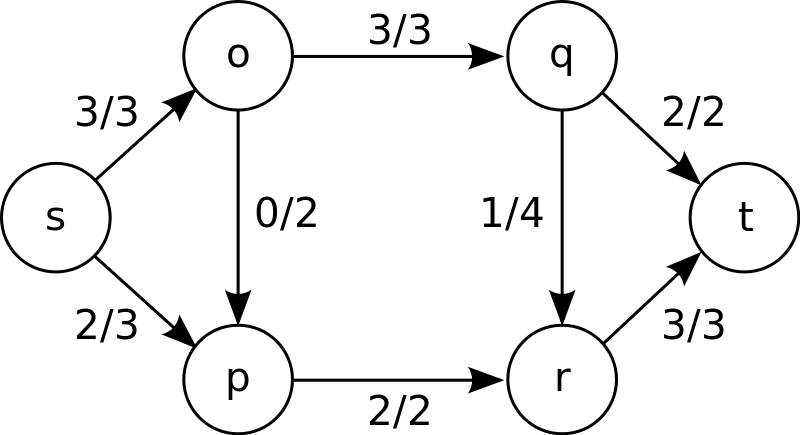
\includegraphics[width=.55\textwidth]{../img/maxflow_wiki}
  \end{center}

  %% TODO: Make my own image here.

  \begin{block}{}
    This image describes the \structure{MAX FLOW} problem. It is part
    of a family of graph problems called \structure{``flow
      problems''}.
  \end{block}}

  \hfill{\tiny Image CC-BY-SA 3.0 by Maksim}
\end{frame}

\begin{frame}
  \frametitle{Network Flow}
  \begin{center}
    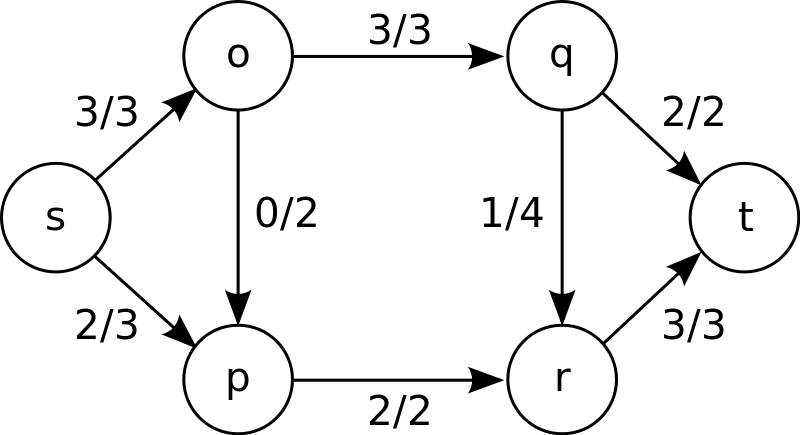
\includegraphics[width=.55\textwidth]{../img/maxflow_wiki}
  \end{center}
  
  {\smaller
    In the image above, \structure{5 ``flow''} go from $s$ to $t$.
    \begin{itemize}
    \item 2 flow go through: $s\rightarrow o\rightarrow q\rightarrow t$;
    \item 1 flow go through: $s\rightarrow o\rightarrow q\rightarrow r\rightarrow t$;
    \item 2 flow go through: $s\rightarrow p\rightarrow r\rightarrow t$;
    \end{itemize}
  }

  \hfill{\tiny Image CC-BY-SA 3.0 by Maksim}
\end{frame}


\begin{frame}[fragile,singleslide]
  \frametitle{Ford Fulkerson Method}

  {\smaller
  \begin{block}{}
    One way to solve the Max Flow problem is using the \structure{Ford-Fulkerson Method}.

    \hfill {\tiny Note: Same Ford as in Bellman-Ford}
  \end{block}
  
  \medskip

  Basic Idea:
  \begin{enumerate}
  \item Create \structure{residual graph} with flow capacity between nodes;
  \item Initial residual graph = weight graph. Non existing edges have capacity 0;
  \item Find a path between $s$ and $t$;
  \item \alert{Remove value} of lowest weight from all edges in residual graph;
  \item \alert{Add value} of lowest weight to all reverse edges in residual graph;
  \item goto 3;
  \end{enumerate}}
\end{frame}

\begin{frame}[fragile,singleslide]
  \frametitle{Ford Fulkerson -- Pseudocode}
{\smaller
  \begin{exampleblock}{}
\begin{verbatim}
int residual[V][V];
memset(residual,0,sizeof(residual))
for (int i; i < AdjList.size();i++)
   for (int j; j < AdjList[i].size();j++)
      residual[i][AdjList[i][j].target] = 
         AdjList[i][j].weight;

mf = 0;
while (P = FindPath(s,t)) > 0) {
   m = P.weight; // minimum edge in P
   for (v in P) {
      residual[v.first][v.second] -= m;
      residual[v.second][v.first] += m;}
   mf += m;
}
\end{verbatim}
  \end{exampleblock}
}
\end{frame}


\begin{frame}[fragile,singleslide]
  \frametitle{Ford Fulkerson Implementation: Finding Paths}

  {\smaller
    \begin{block}{}
\begin{verbatim}
while (P = FindPath(s,t) > 0) {...}
\end{verbatim}

A key part of the algorithm is finding paths from $s$ to $t$, and
calculating the flow of the path (minimum edge weigth). We can use any
algorithm to implement this search.
    \end{block}

\begin{exampleblock}{Idea 1: Find augmenting paths using DFS;}
  This is simple to implement, but the worst case scenario has cost:
  $O(|f*|E)$, where $f*$ is the true Max Flow value.

  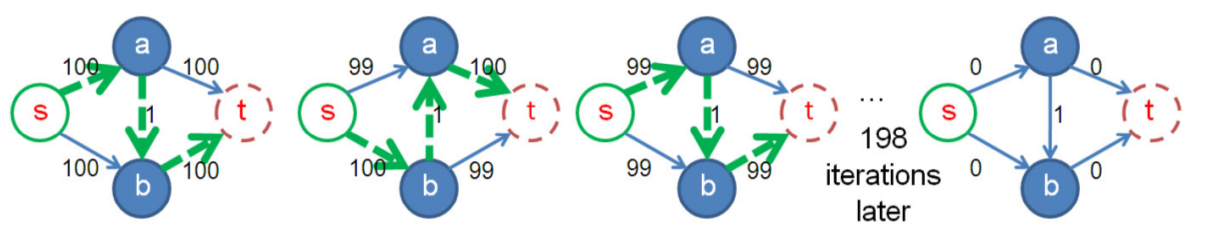
\includegraphics[width=1\textwidth]{../img/ff_worst_halim}

\end{exampleblock}
}
\hfill{\tiny Image from Competitive Programming, 3rd edition}
\end{frame}

\begin{frame}[fragile,singleslide]
  \frametitle{Edmond Karp's Algorithm}

  {\smaller
  \begin{block}{O(|f*|E) is too expensive!}
    The algorithm presented in the last page is too expensive for
    arbitrary values of |f*|. The \structure{Edmond Karp} algorithm is 
    a $O(VE^2)$ variation using BFS.
  \end{block}

\begin{verbatim}
//// PART 1: Augment based on BFS

// This is a simpler O(V^3E) implementation
int res[MAX_V][MAX_V], mf, s, t;
vi p; // BFS spanning tree from s

void augment(int v, int minEdge) { // traverse BFS s->t
   inf (v == s) { f = minEdge; return; }
   else if (p[v] != -1) { 
      augment(p[v], min(minEdge,res[p[v]][v]));
      res[p[v]][v] -= f; res[v][p[v]] += f;}}
\end{verbatim}
}
\end{frame}

\begin{frame}[fragile,singleslide]
  \frametitle{Edmond Karp's Algorithm (2)}
  {\smaller
  \begin{block}{O(|f*|E) is too expensive!}
    The algorithm presented in the last page is too expensive for
    arbitrary values of |f*|. The \structure{Edmond Karp} algorithm is 
    a $O(VE^2)$ variation using BFS.
  \end{block}

\begin{verbatim}
//// PART 2: create the BFS
mf = 0;
while (1) { f = 0; vi dist(MAX_V,INF): dist[s] = 0;
            queue<int> q; q.push(s); p.assign(MAX_V,-1);
   while (!q.empty()) { int u = q.front; q.pop();
      if (u==t) break; for int (v = 0; v < MAX_V; v++)
         if (res[u][v] > 0 && dist[v] == INF)
            dist[v] = dist[u]+1, q.push(v), p[v] = u; }
   // BFS (parent indexes) is now in "p";
   augment(t,INF); // modify residuals based on P
   if (f == 0) break; // if no more flow, end.
   mf += f;
   }
\end{verbatim}
  }
\end{frame}

\subsection{Problem Sample 1}
\begin{frame}
  \frametitle{NF Example: UVA 259 -- Software Allocation}
  
  {\smaller
    \begin{block}{Problem Description}
      \begin{itemize}
      \item (up to) 26 programs and 10 computers;
      \item Each computer can run only one program at a time;
      \item Each computer has a list of programs it can run;
      \item Each program wants to run in ``p'' computers;
      \end{itemize}
      Can you find an allocation to run all programs?
    \end{block}

    \bigskip
    
    \structure{Allocation Problems} (Often called ``matching''
    problems) can be solved using the Max Flow algorithm. 

    \smallskip

    Create a \structure{source} node connected to all the requesters;
    and an \structure{end} node connected to all the providers. The
    max flow between the source and the end shows how much of the
    allocation is possible.
    }
\end{frame}

\begin{frame}[fragile,singleslide]
  \frametitle{NF Example: UVA 259 -- Software Allocation}




  {\smaller
\begin{verbatim}
A4 01345;
Q1 6
P4 35789;
\end{verbatim}


   \begin{center}
     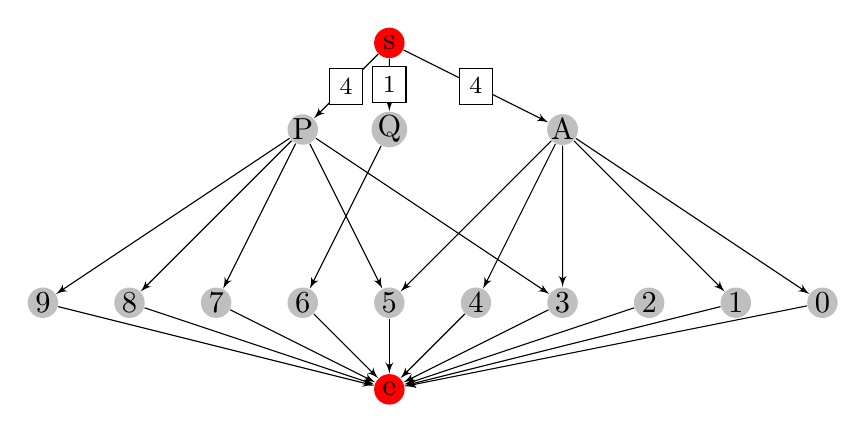
\begin{tikzpicture}[transform shape,label/.style={thin, draw=black, align=center,fill=white,font=\smaller},scale=1.1]
       \tikzset{edge/.style = {->,>=latex'}}
       \node[red vertex] (s) at (0,0) {s};
       \node[vertex] (A) at (2,-1) {A};
       \node[vertex] (Q) at (0,-1) {Q};
       \node[vertex] (P) at (-1,-1) {P};
       \node[vertex] (0) at (5,-3) {0};
       \node[vertex] (1) at (4,-3) {1};
       \node[vertex] (2) at (3,-3) {2};
       \node[vertex] (3) at (2,-3) {3};
       \node[vertex] (4) at (1,-3) {4};
       \node[vertex] (5) at (0,-3) {5};
       \node[vertex] (6) at (-1,-3) {6};
       \node[vertex] (7) at (-2,-3) {7};
       \node[vertex] (8) at (-3,-3) {8};
       \node[vertex] (9) at (-4,-3) {9};
       \node[red vertex] (e) at (0,-4) {e};
       \draw[edge] (s) -- node[label] {4} (A);
       \draw[edge] (s) -- node[label] {1} (Q);
       \draw[edge] (s) -- node[label] {4} (P);
       \draw[edge] (A) -- (0);
       \draw[edge] (A) -- (1);
       \draw[edge] (A) -- (5);
       \draw[edge] (A) -- (3);
       \draw[edge] (A) -- (4);
       \draw[edge] (Q) -- (6);
       \draw[edge] (P) -- (5);
       \draw[edge] (P) -- (3);
       \draw[edge] (P) -- (7);
       \draw[edge] (P) -- (8);
       \draw[edge] (P) -- (9);
       \draw[edge] (0) -- (e);
       \draw[edge] (1) -- (e);
       \draw[edge] (2) -- (e);
       \draw[edge] (3) -- (e);
       \draw[edge] (4) -- (e);
       \draw[edge] (5) -- (e);
       \draw[edge] (6) -- (e);
       \draw[edge] (7) -- (e);
       \draw[edge] (8) -- (e);
       \draw[edge] (9) -- (e);
     \end{tikzpicture}
   \end{center}
  }
\end{frame}

\subsection{Problem Variants}
\begin{frame}
  \frametitle{Network Flow Problem Variants (1)}
  {\smaller
  \begin{block}{Minimum Cut -- UVA 10480 (Sabotage)}
    Find a minimum set of edges C so that if all edges from the set
    are removed, then the flow from $s$ to $e$ becomes 0. (i.e., $s$
    and $e$ are disconnected).
  \end{block}

  Ideas:
  \begin{itemize}
  \item Perform the Max Flow, and analyse the residual matrix;
  \item All nodes reachable from $s$ using edges with positive
    residual are connected to $s$;
  \item All nodes not reachable from $s$ as above are connected to $e$;
  \item All edges with residual $0$ connect the two sets, and belong
    to the Minimum Cut;
  \end{itemize}
  }
\end{frame}

\begin{frame}
  \frametitle{Network Flow Problem Variants (2)}
  {\smaller
    \begin{block}{Multiple Sources, Multiple Sinks}
    \end{block}

    Ideas:
    \begin{itemize}
    \item Create a ``super source'' node ss. ss connects to all sources with infinite weight;
    \item Create a ``super sink'' node se. All sinks connect to se with infinite weight;
    \end{itemize}

    \begin{block}{Weights on nodes, not edges}
    \end{block}
    Ideas:
    \begin{itemize}
    \item Split the vertices. Vertice weight is now an edge connecting both halves.
    \item Be careful. Doing this doubles V and increases E.
    \item (note how many times the solution is to modify the graph to our needs)
    \end{itemize}

    %% TODO: Add example problems for these cases
  }
\end{frame}

\section{Special Graphs}
\subsection{Special Graphs}
% TODO: Replaced ``bipartite Match'' with special graphs, deal with many examples from 4.7.*

\begin{frame}
  \frametitle{Graph Problems: Thinking with many boxes} 
  
  {\smaller
  The interesting part about graph problems is that they came in great
  variety. Once you know the basic algorithms, the main problem is figuring
  out what kind of graph you are dealing with.

  This knowlege only comes with practice, but here are some examples.
  }
\end{frame}

\subsection{Fishmonger}

\begin{frame}
  \frametitle{DAG example: Fishmonger (SPOJ 0101)}
  {\smaller
  \begin{block}{Problem Description}
    You are given a number of cities $3\leq n \leq 50$, remaining time
    $1 \leq t \leq 1000$, a toll matrix and a travel time matrix,
    choose a route:
    \begin{itemize}
    \item starting at city $0$ and ending at city $n-1$;
    \item travel time must be less than $t$;
    \item toll must be minimum;
    \end{itemize}
  \end{block}

  \bigskip

  There are two goals: \emph{time} and \emph{cost} that can contradict
  each other. How do you calculate the SSSP in this condition?
  }
\end{frame}

\begin{frame}
  \frametitle{DAG example: Fishmonger (SPOJ 0101)} 

  To handle the time constraint, we add a parameter (state) to each
  vertex indicating how much time is left.

  \bigskip

  The number of nodes will be multiplied: $(1) \leftarrow (1,t),
  (1,t-1),(1,t-2),\ldots,(1,0)$,\\ but now the graph is an DAG (time can
  only move in one direction).

  \bigskip

  But because it is a DAG, the problem becomes solvable using DP
  search (\emph{find(city,timeleft)}).
\end{frame}


\subsection{Titanic}
\begin{frame}[fragile,singleslide]
  \frametitle{Network Flow Example 2: Titanic (UVA 11380)}

  {\smaller
  \begin{block}{Problem Description}
    You are given a map of an accident:

\begin{verbatim}
# -- large wood: safe place, houses P people;
@ -- large iceberg: unsafe, houses 1 person;
. -- ice: unsafe, 1 person, breaks after using once;
~ -- freezing water: unsafe, no one can use;
* -- initial position of each person;
\end{verbatim}
    How many people can find paths to the safe place?
  \end{block}
  \begin{center}
    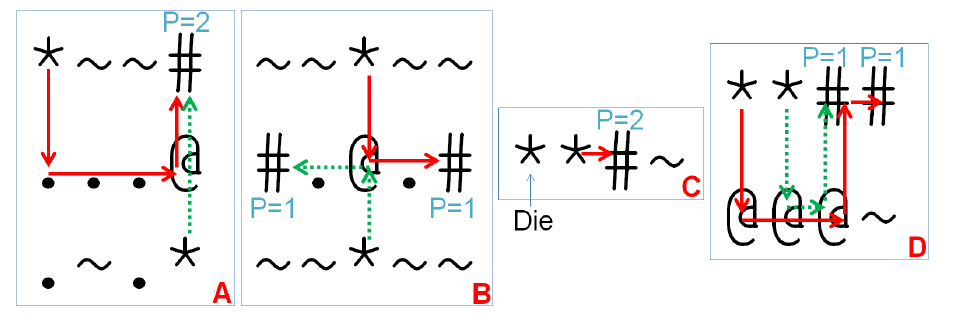
\includegraphics[width=0.7\textwidth]{../img/uva11380_halim}
  \end{center}
  \hfill{\tiny Image from \emph{Competitive Programming, 3rd edition}}
  }
\end{frame}

\begin{frame}
  \frametitle{Network Flow Example 2: Titanic (UVA11380)}
  {\smaller
  \begin{block}{Graph Modeling}
    Since we have many people trying to go to the safe places, we can
    model this problem as a Max Flow problem. How do we set up the graph?
  \end{block}
  \uncover<2>{
  \begin{itemize}
  \item Connect all non ``water'' cells with INF capacity to represent the paths;
  \item Set vertex capacity: ice and initial position is 1, iceberg
    and large wood is INF, to represent breaking;
  \item Super source node connect to all survivors with capacity 1;
  \item Super sink node connect to all large woods with capacity P;
  \end{itemize}}
  }
\end{frame}

\subsection{Prime Pairing}
\begin{frame}
  \frametitle{Bipartite Example - Prime pairing}
  \begin{block}{Problem Description}
    Two numbers $a,b$ can be \structure{prime paired} if their sum
    $a+b$ is prime. Given a set of numbers $N$, print the pairings of
    $N[0]$ that allow a \structure{complete pairing} of $N$ to be
    made.
  \end{block}

  Examples:  
  \begin{itemize}
  \item $N = \{1,4,7,10,11,12\}$ -- answer: $\{4,10\}$
  \end{itemize}

  \vfill

  Is this even a graph problem??
\end{frame}

\begin{frame}
  \frametitle{Bipartite Example - Prime pairing}
  \begin{block}{}
    The trick is to note that this is an ``allocation'' problem, just
    like ``software allocation''. Each number will be allocated to
    another number to form primes.
  \end{block}

  How to create the graph:
  \begin{itemize}
  \item Split set between odds and evens (because odd + odd is not prime);
  \item Create edges between odds and evens that sum primes;
  \item super source connects to odds, super sink connects to edges;
  \item see if the max flow is equal to the number of nodes/2;
  \end{itemize}
\end{frame}

%\begin{frame}
%  \frametitle{Flow and Special Graph problems}
% %% TODO: Add more special problems from the book for discussion
%\end{frame}

\section{Conclusion}
\subsection{Conclusion}
\begin{frame}
  \frametitle{Summary}
  \begin{itemize}
  \item BFS for unweighted path search; Djikstra for weighted path search;
  \item Bellman-ford for weighted path search with negative loops;
  \item Floyd-Warshall for all-to-all path search;
  \item Ford-Fergusson for Network flow

    \bigskip

  \item However, the most important skill in graph problems is knowing
    how to transform the problem into a graph that can be solved by a
    known algorithm;
  \end{itemize}
\end{frame}

\begin{frame}
  \frametitle{This Week's Problems}
  {\smaller
  \begin{itemize}
    \item From Dusk Until Down;
    \item Wormholes; 
    \item Mice and Maze; 
    \item Degrees of Separation;
    \item Avoiding your Boss;
    \item Arbitrage;
    \item \alert{Software Allocation};
    \item \alert{Sabotage};
    \item \alert{Little Red Riding Hood};
    \item \alert{Gopher II};
  \end{itemize}}
\end{frame}

\begin{frame}
  \frametitle{Next Weeks}
  \begin{itemize}
  \item Week 7 -- Math Problems;
  \item Week 8 -- Computational Geometry;
  \item Week 9 -- String Problems;
  \end{itemize}

  \vfill
  
  Hang in there a little bit more! :-)
  
\end{frame}

\end{document}

